% Options for packages loaded elsewhere
% Options for packages loaded elsewhere
\PassOptionsToPackage{unicode}{hyperref}
\PassOptionsToPackage{hyphens}{url}
\PassOptionsToPackage{dvipsnames,svgnames,x11names}{xcolor}
%
\documentclass[
  letterpaper,
  DIV=11,
  numbers=noendperiod]{scrartcl}
\usepackage{xcolor}
\usepackage{amsmath,amssymb}
\setcounter{secnumdepth}{-\maxdimen} % remove section numbering
\usepackage{iftex}
\ifPDFTeX
  \usepackage[T1]{fontenc}
  \usepackage[utf8]{inputenc}
  \usepackage{textcomp} % provide euro and other symbols
\else % if luatex or xetex
  \usepackage{unicode-math} % this also loads fontspec
  \defaultfontfeatures{Scale=MatchLowercase}
  \defaultfontfeatures[\rmfamily]{Ligatures=TeX,Scale=1}
\fi
\usepackage{lmodern}
\ifPDFTeX\else
  % xetex/luatex font selection
  \setmainfont[]{Verdana}
  \setsansfont[]{Verdana}
\fi
% Use upquote if available, for straight quotes in verbatim environments
\IfFileExists{upquote.sty}{\usepackage{upquote}}{}
\IfFileExists{microtype.sty}{% use microtype if available
  \usepackage[]{microtype}
  \UseMicrotypeSet[protrusion]{basicmath} % disable protrusion for tt fonts
}{}
\makeatletter
\@ifundefined{KOMAClassName}{% if non-KOMA class
  \IfFileExists{parskip.sty}{%
    \usepackage{parskip}
  }{% else
    \setlength{\parindent}{0pt}
    \setlength{\parskip}{6pt plus 2pt minus 1pt}}
}{% if KOMA class
  \KOMAoptions{parskip=half}}
\makeatother
% Make \paragraph and \subparagraph free-standing
\makeatletter
\ifx\paragraph\undefined\else
  \let\oldparagraph\paragraph
  \renewcommand{\paragraph}{
    \@ifstar
      \xxxParagraphStar
      \xxxParagraphNoStar
  }
  \newcommand{\xxxParagraphStar}[1]{\oldparagraph*{#1}\mbox{}}
  \newcommand{\xxxParagraphNoStar}[1]{\oldparagraph{#1}\mbox{}}
\fi
\ifx\subparagraph\undefined\else
  \let\oldsubparagraph\subparagraph
  \renewcommand{\subparagraph}{
    \@ifstar
      \xxxSubParagraphStar
      \xxxSubParagraphNoStar
  }
  \newcommand{\xxxSubParagraphStar}[1]{\oldsubparagraph*{#1}\mbox{}}
  \newcommand{\xxxSubParagraphNoStar}[1]{\oldsubparagraph{#1}\mbox{}}
\fi
\makeatother


\usepackage{longtable,booktabs,array}
\newcounter{none} % for unnumbered tables
\usepackage{calc} % for calculating minipage widths
% Correct order of tables after \paragraph or \subparagraph
\usepackage{etoolbox}
\makeatletter
\patchcmd\longtable{\par}{\if@noskipsec\mbox{}\fi\par}{}{}
\makeatother
% Allow footnotes in longtable head/foot
\IfFileExists{footnotehyper.sty}{\usepackage{footnotehyper}}{\usepackage{footnote}}
\makesavenoteenv{longtable}
\usepackage{graphicx}
\makeatletter
\newsavebox\pandoc@box
\newcommand*\pandocbounded[1]{% scales image to fit in text height/width
  \sbox\pandoc@box{#1}%
  \Gscale@div\@tempa{\textheight}{\dimexpr\ht\pandoc@box+\dp\pandoc@box\relax}%
  \Gscale@div\@tempb{\linewidth}{\wd\pandoc@box}%
  \ifdim\@tempb\p@<\@tempa\p@\let\@tempa\@tempb\fi% select the smaller of both
  \ifdim\@tempa\p@<\p@\scalebox{\@tempa}{\usebox\pandoc@box}%
  \else\usebox{\pandoc@box}%
  \fi%
}
% Set default figure placement to htbp
\def\fps@figure{htbp}
\makeatother





\setlength{\emergencystretch}{3em} % prevent overfull lines

\providecommand{\tightlist}{%
  \setlength{\itemsep}{0pt}\setlength{\parskip}{0pt}}



 


\usepackage{booktabs}
\usepackage{longtable}
\usepackage{array}
\usepackage{multirow}
\usepackage{wrapfig}
\usepackage{float}
\usepackage{colortbl}
\usepackage{pdflscape}
\usepackage{tabu}
\usepackage{threeparttable}
\usepackage{threeparttablex}
\usepackage[normalem]{ulem}
\usepackage{makecell}
\usepackage{xcolor}
\KOMAoption{captions}{tableheading}
\makeatletter
\@ifpackageloaded{caption}{}{\usepackage{caption}}
\AtBeginDocument{%
\ifdefined\contentsname
  \renewcommand*\contentsname{Table of contents}
\else
  \newcommand\contentsname{Table of contents}
\fi
\ifdefined\listfigurename
  \renewcommand*\listfigurename{List of Figures}
\else
  \newcommand\listfigurename{List of Figures}
\fi
\ifdefined\listtablename
  \renewcommand*\listtablename{List of Tables}
\else
  \newcommand\listtablename{List of Tables}
\fi
\ifdefined\figurename
  \renewcommand*\figurename{Figure}
\else
  \newcommand\figurename{Figure}
\fi
\ifdefined\tablename
  \renewcommand*\tablename{Table}
\else
  \newcommand\tablename{Table}
\fi
}
\@ifpackageloaded{float}{}{\usepackage{float}}
\floatstyle{ruled}
\@ifundefined{c@chapter}{\newfloat{codelisting}{h}{lop}}{\newfloat{codelisting}{h}{lop}[chapter]}
\floatname{codelisting}{Listing}
\newcommand*\listoflistings{\listof{codelisting}{List of Listings}}
\makeatother
\makeatletter
\makeatother
\makeatletter
\@ifpackageloaded{caption}{}{\usepackage{caption}}
\@ifpackageloaded{subcaption}{}{\usepackage{subcaption}}
\makeatother
\usepackage{bookmark}
\IfFileExists{xurl.sty}{\usepackage{xurl}}{} % add URL line breaks if available
\urlstyle{same}
\hypersetup{
  pdftitle={Niobrara Housing Study},
  colorlinks=true,
  linkcolor={blue},
  filecolor={Maroon},
  citecolor={Blue},
  urlcolor={Blue},
  pdfcreator={LaTeX via pandoc}}


\title{Niobrara Housing Study}
\author{Bobbi Pettit, AICP \and Jordan Duffin Wong, Ph.D}
\date{}
\begin{document}
\maketitle


\subsection*{Purpose}\label{purpose}
\addcontentsline{toc}{subsection}{Purpose}

Upon completion of the Study, the community's leadership and housing
stakeholders should move forward by continuing to take the following
steps.

\begin{enumerate}
\def\labelenumi{(\arabic{enumi})}
\tightlist
\item
  Seek Partnerships: Continue working with other agencies,
  organizations, and neighboring jurisdictions to leverage resources.
\item
  Explore Funding Opportunities: The Federal and State governments
  understand that the lack of affordable housing is affecting the entire
  country. As such, Federal and State programs continue to be made
  available to governments committed to solving housing problems on a
  local scale. With the knowledge of the state of their community, they
  must stay informed about programs that provide financial resources or
  incentives for affordable housing and infrastructure improvements.
\item
  Recognize Achievements and Share Best Practices: Recognize and
  celebrate successful housing development initiatives within the
  community. Share best practices, lessons learned, and success stories
  with other cities and regions to promote knowledge sharing,
  collaborative learning, and mutual growth.
\end{enumerate}

\subsection*{Process}\label{process}
\addcontentsline{toc}{subsection}{Process}

The Housing Study documents the conditions, statuses, and needs for
housing in Niobrara. Drawing on a variety of data from the Knox County,
Nebraska Property Assessor, various government agencies, and original
surveys of Niobrara residents, we show that Niobrara has a long-term
trend of population decline and housing structures in need of
improvement.

\subsection*{Housing Condition and Age}\label{housing-condition-and-age}
\addcontentsline{toc}{subsection}{Housing Condition and Age}

The status and the condition of the residential structures in Knox
County are documented by the Knox County Property Assessor. They use
five ratings:\footnote{The Assessor also calculates intermediate
  ratings, e.g.~``Worn Out - Badly Worn.''}

\begin{enumerate}
\def\labelenumi{\arabic{enumi}.}
\item
  \textbf{Worn Out}: homes that are in a state of severe disrepair or
  uninhabitable condition.
\item
  \textbf{Badly Worn}: homes that have serious deficiencies in systems,
  such as roofing, plumbing, or electrical foundation. They also show
  visible deterioration.
\item
  \textbf{Average}: homes that are habitable and maintain a standard
  level of functionality. They may lack modern updates or show signs of
  aging and general wear.
\item
  \textbf{Good}: homes that are newer, well-maintained, or recently
  renovated.
\item
  \textbf{Very Good}: homes that are extremely new, extremely
  well-maintained, and feature modern amenities and features.
\end{enumerate}

The map below displays the housing conditions in Niobrara.

\begin{center}
\pandocbounded{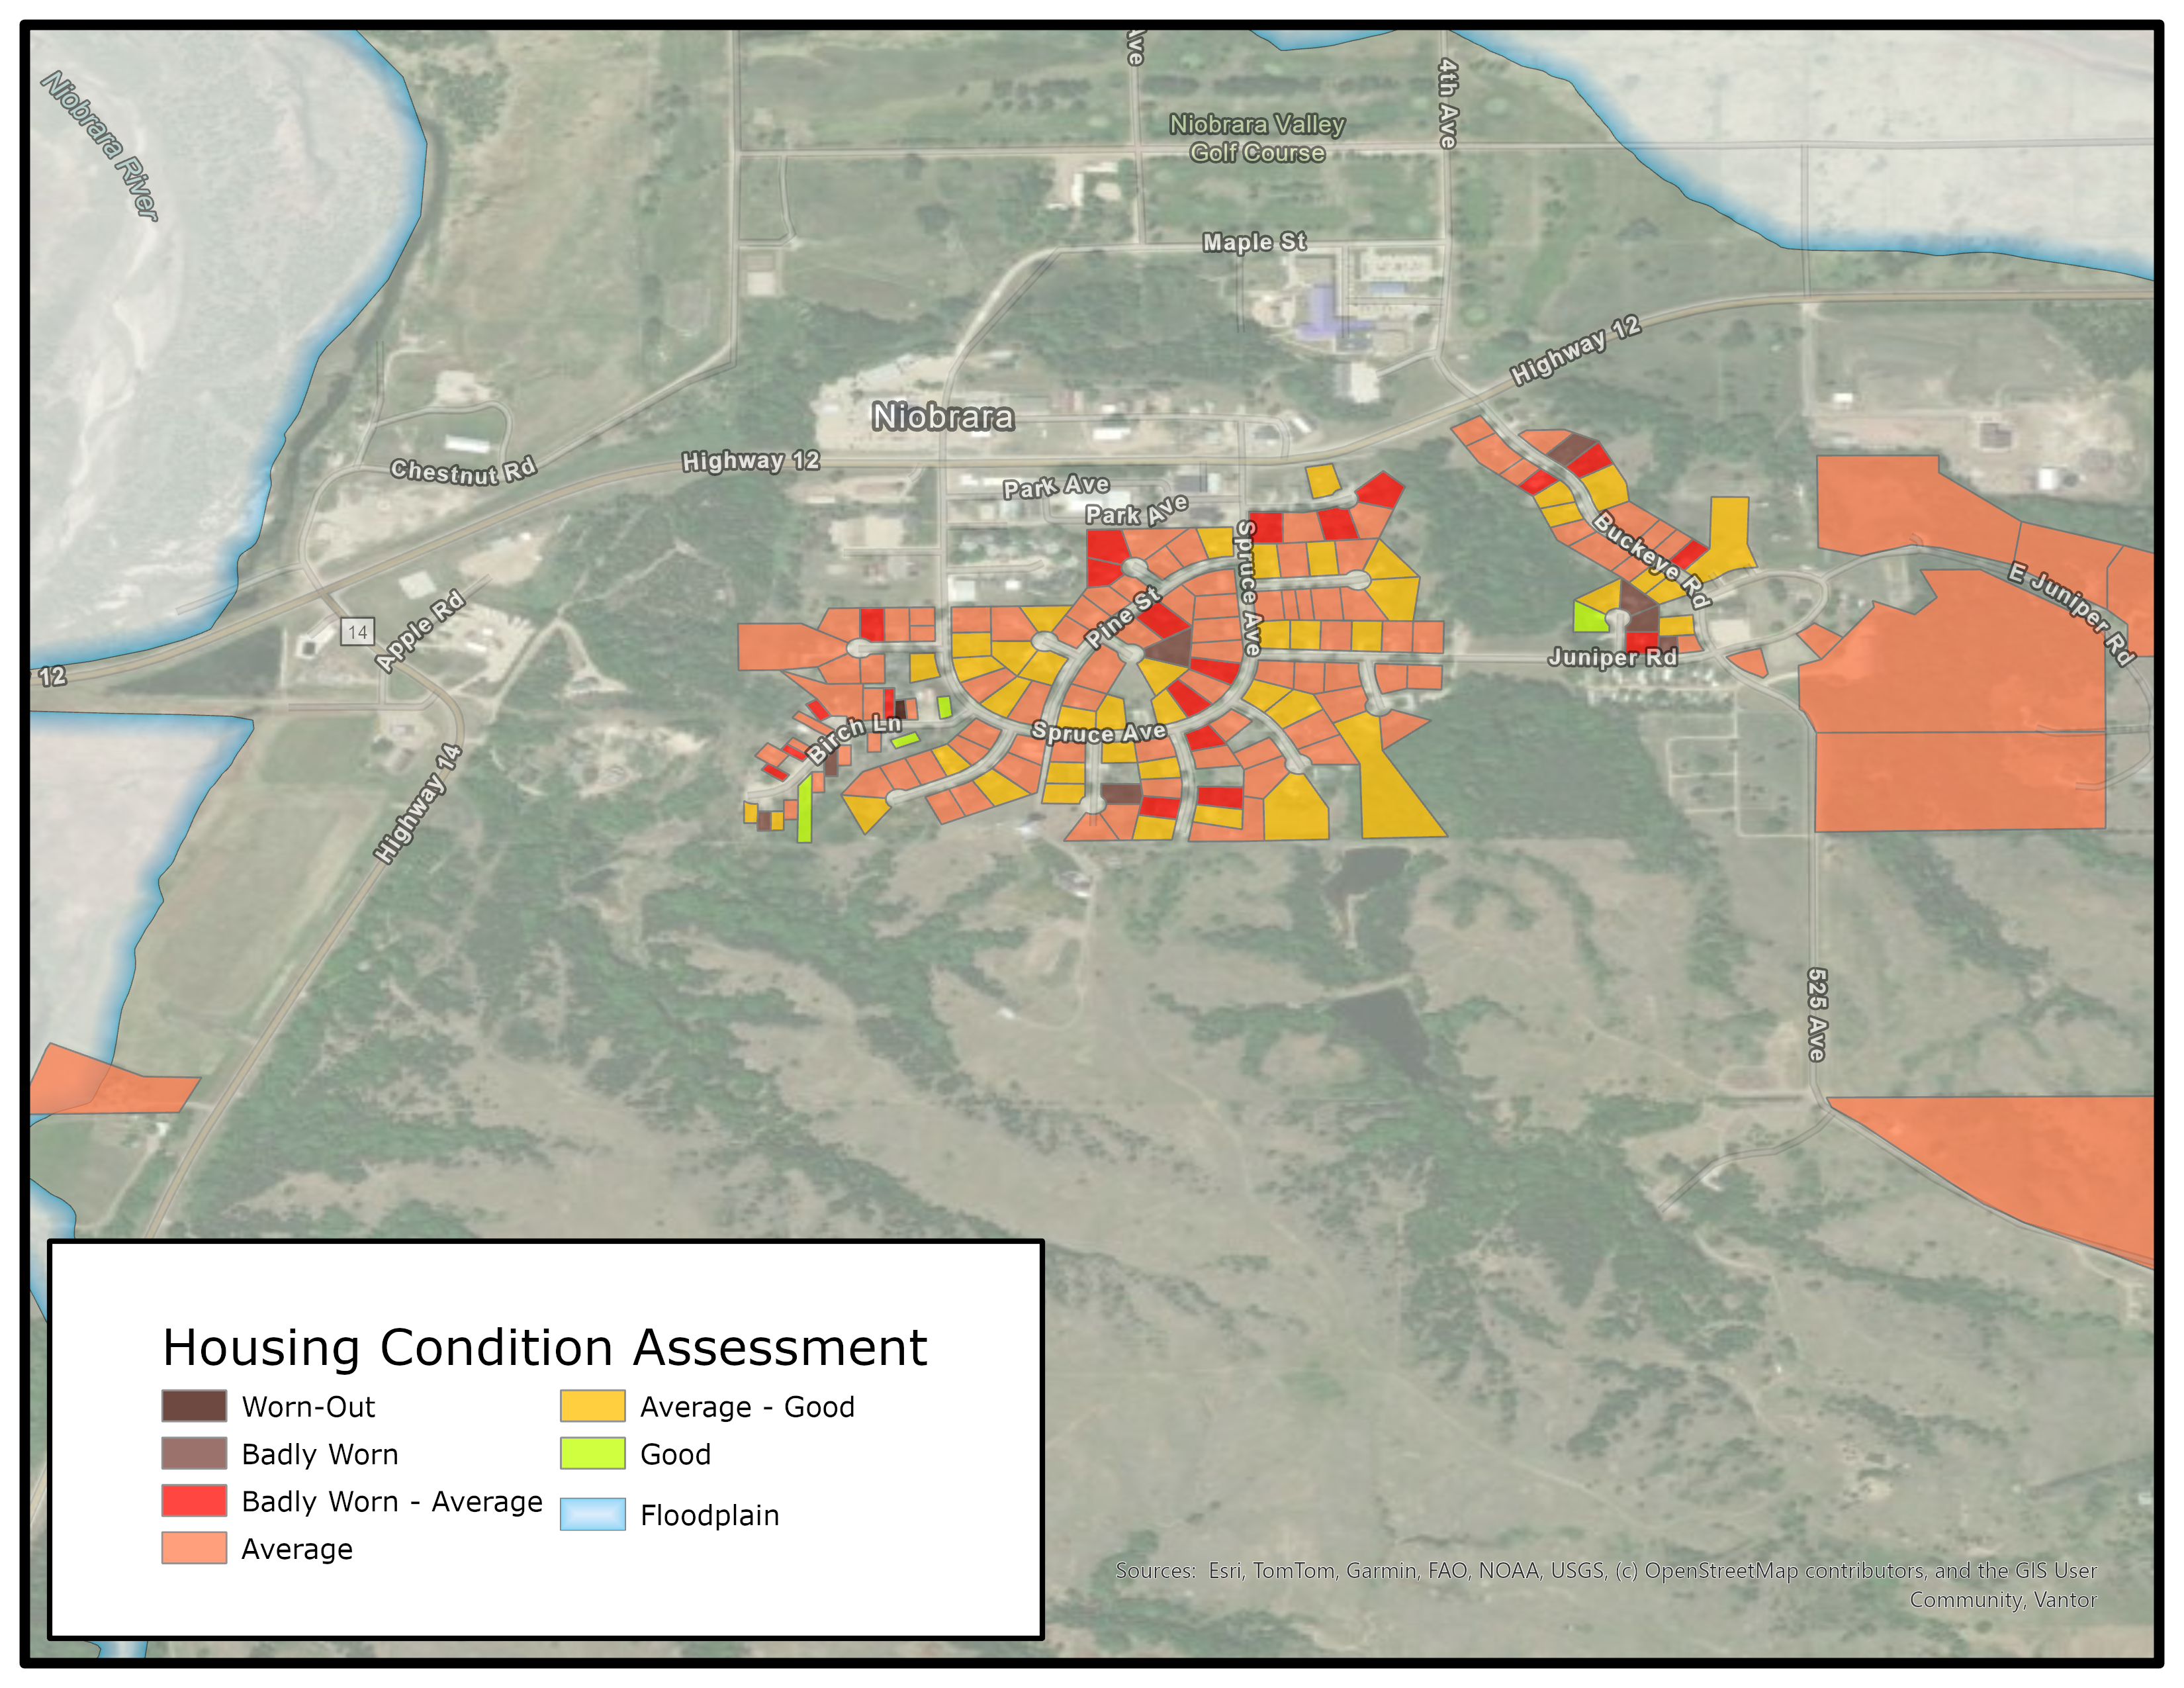
\includegraphics[keepaspectratio]{figures/housing_condition.png}}
\end{center}

\begin{longtable*}[l]{lc>{\centering\arraybackslash}p{12em}c}
\toprule
\cellcolor{gray}{\textcolor{white}{Condition}} & \cellcolor{gray}{\textcolor{white}{Parcels}} & \cellcolor{gray}{\textcolor{white}{Area (Square Acres)}} & \cellcolor{gray}{\textcolor{white}{Percent of Total Area}}\\
\midrule
\endfirsthead
\multicolumn{4}{@{}l}{\textit{(continued)}}\\
\toprule
\cellcolor{gray}{\textcolor{white}{Condition}} & \cellcolor{gray}{\textcolor{white}{Parcels}} & \cellcolor{gray}{\textcolor{white}{Area (Square Acres)}} & \cellcolor{gray}{\textcolor{white}{Percent of Total Area}}\\
\midrule
\endhead

\endfoot
\bottomrule
\endlastfoot
\cellcolor{gray!10}{Worn-Out} & \cellcolor{gray!10}{1} & \cellcolor{gray!10}{1.00} & \cellcolor{gray!10}{0.07\%}\\
Badly Worn & 8 & 21.91 & 1.44\%\\
\cellcolor{gray!10}{Badly Worn - Average} & \cellcolor{gray!10}{20} & \cellcolor{gray!10}{64.97} & \cellcolor{gray!10}{4.28\%}\\
Average & 100 & 1,211.72 & 79.76\%\\
\cellcolor{gray!10}{Average - Good} & \cellcolor{gray!10}{43} & \cellcolor{gray!10}{209.92} & \cellcolor{gray!10}{13.82\%}\\
\addlinespace
Good & 4 & 9.65 & 0.64\%\\*
\end{longtable*}

We have several remarks on the housing conditions in Niobrara:

\begin{enumerate}
\def\labelenumi{\arabic{enumi}.}
\tightlist
\item
  The overwhelming majority of housing is in \textbf{average} condition:

  \begin{itemize}
  \tightlist
  \item
    About \textbf{80\%} of the homes in Niobrara are habitable and
    maintain a standard level of functionality. However, they may lack
    modern updates or show signs of aging and general wear.
  \end{itemize}
\item
  Very few homes are \textbf{worn out}:

  \begin{itemize}
  \item
    Only \textbf{one} home is in a state of severe disrepair or
    uninhabitable condition.\footnote{According to the property
      assessor, at least.} This reflects a minimum standard of basic
    housing adequacy in Niobrara, with little evidence of total
    structural abandonment.
  \item
    It also suggests that code enforcement or demolition efforts may be
    effective in preventing extreme blight.
  \end{itemize}
\item
  A very small proportion of houses are \textbf{badly worn}:

  \begin{itemize}
  \item
    About \textbf{1.44\%} of the housing stock is assessed as ``badly
    worn'' or ``badly worn - average.'' These homes may have serious
    deficiencies in systems (such as roofing, plumbing, or electrical
    foundation) or visible deterioration.
  \item
    This group represents homes that are likely still occupied but
    nearing the point where repairs and renovation are critical.
  \end{itemize}
\item
  A similarly small proportion of houses are \textbf{good or better}:

  \begin{itemize}
  \item
    Only about \textbf{14\%} of homes are rated better than ``average,''
    suggesting a small segment of housing stock that is particularly
    well-maintained, or recently renovated. This could indicate limited
    recent investment in high-quality residential development or
    upgrades.
  \item
    It also highlights the need for incentives and programs to support
    home improvement or new building efforts.
  \end{itemize}
\end{enumerate}

\textbf{Overall Implications for Housing Policy}: Niobrara's housing
stock is in reasonably good condition. Niobrara's citizens have done a
good job of maintaining their residences. For the small amount of
housing stock that is rated worse than ``average,'' Niobrara may benefit
from targeted housing rehabilitation programs centered on owner-occupied
homes in poor condition. Grant funding and development efforts can be
focused on preventing the decline of average-rated homes while
prioritizing repairs for the five percent of below-average stock.

The Knox County Property Assessor also documents the age of housing
structures. Knowing the age of community housing stock is important
because the workable lifespan of a typical house is about one hundred
years. Because Niobrara moved to its current location in the 1970s, most
of housing stock is much newer than the stock across the rest of Western
Knox County. Of note:\footnote{See
  \href{https://niobrarane.com/history/}{the Village's History page.}}

\begin{quote}
The mighty Missouri again invaded Niobrara in April of 1952 and much of
the town and the surrounding area was flooded. This record flow came
shortly before the completion of the Missouri River dams, citizens were
relieved that flooding along the Missouri would be a thing of the past
and life could continue at a more or less routine pace.A big event of
the 1950's was the Centennial Celebration of June 16 -- 17, 1956. There
were many events leading up to the two day celebration which was
attended by an estimated 20,000 people. Later, in the 1950's and in the
1960's, it became apparent that the mighty Missouri would, again,
influence Niobrara history. Silt from the Niobrara River, which began to
accumulate in the river bed, raised the ground water level in Niobrara
and the surrounding area. Many basements became flooded requiring
constant pumping and it was apparent that the problem would continue to
intensify. By 1969, community officials began to look for solutions and
a second move.

Funds were appropriated by Congress to pay a sizable portion of the cost
of the move.~Site preparation began in September of 1973 and was
completed in April of 1974. Next came the water, sewer, storm sewer,
paving, water wells and water storage tank. The sale of residential lots
followed~ in the summer of 1974 and residential construction moved
forward at a fast pace. By the end of 1977, the move was nearly
completed. The 1980 census showed 420 and 213 homes in Niobrara.~1981
marked the 112th anniversary of the original settlement and was
celebrated with a historical pageant, parade and other activitiesThrough
volunteer efforts, a nine-hole grass greens golf course was completed on
the old town site. The Niobrara State Park was relocated, suffering the
same fate as the old town.~Niobrara's history can best be summarized as
being destined by the mighty Missouri on whose banks it was founded and
from whose reach it has continuously tried to escape.
\end{quote}

\begin{center}
\pandocbounded{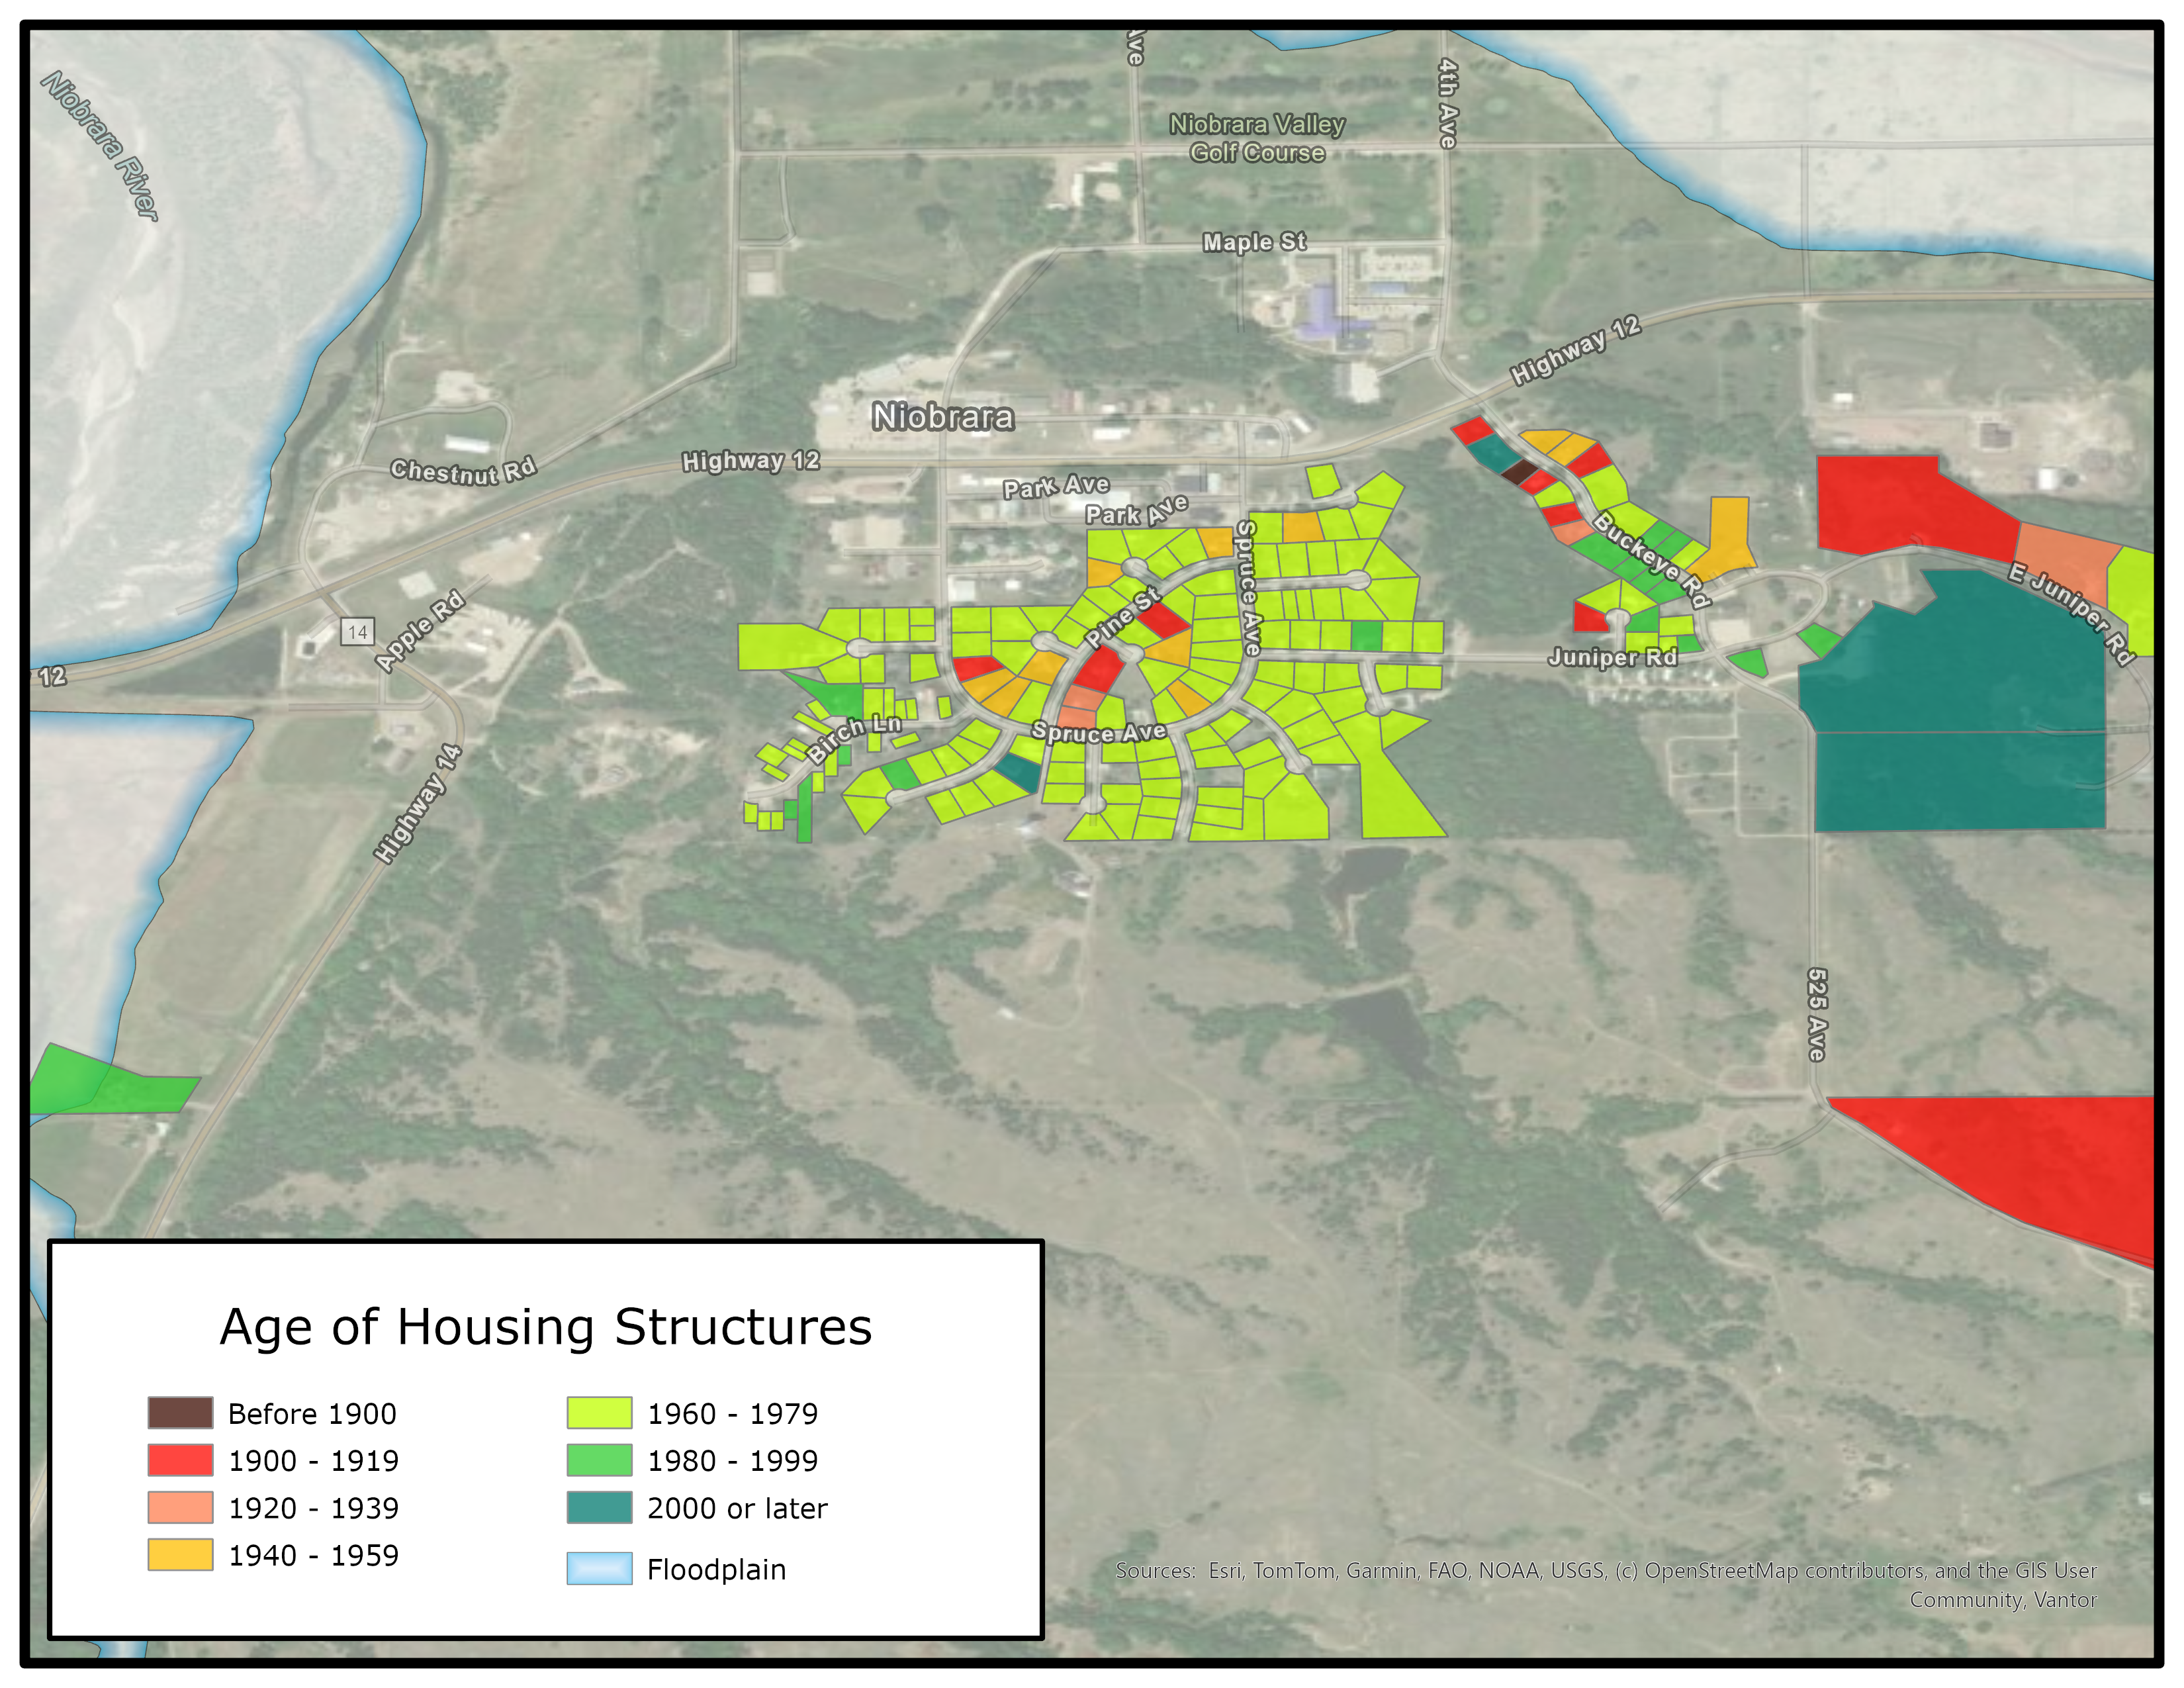
\includegraphics[keepaspectratio]{figures/housing_age.png}}
\end{center}

\begin{longtable*}[l]{lc>{\centering\arraybackslash}p{12em}c}
\toprule
\cellcolor{gray}{\textcolor{white}{Decade Built}} & \cellcolor{gray}{\textcolor{white}{Parcels}} & \cellcolor{gray}{\textcolor{white}{Area (Square Acres)}} & \cellcolor{gray}{\textcolor{white}{Percent of Total Area}}\\
\midrule
\endfirsthead
\multicolumn{4}{@{}l}{\textit{(continued)}}\\
\toprule
\cellcolor{gray}{\textcolor{white}{Decade Built}} & \cellcolor{gray}{\textcolor{white}{Parcels}} & \cellcolor{gray}{\textcolor{white}{Area (Square Acres)}} & \cellcolor{gray}{\textcolor{white}{Percent of Total Area}}\\
\midrule
\endhead

\endfoot
\bottomrule
\endlastfoot
\cellcolor{gray!10}{Before 1900} & \cellcolor{gray!10}{1} & \cellcolor{gray!10}{2.47} & \cellcolor{gray!10}{0.16\%}\\
1900 - 1919 & 10 & 248.90 & 16.38\%\\
\cellcolor{gray!10}{1920 - 1939} & \cellcolor{gray!10}{4} & \cellcolor{gray!10}{32.93} & \cellcolor{gray!10}{2.17\%}\\
1940 - 1959 & 11 & 55.86 & 3.68\%\\
\cellcolor{gray!10}{1960 - 1979} & \cellcolor{gray!10}{126} & \cellcolor{gray!10}{511.32} & \cellcolor{gray!10}{33.66\%}\\
\addlinespace
1980 - 1999 & 18 & 87.25 & 5.74\%\\
\cellcolor{gray!10}{2000 or later} & \cellcolor{gray!10}{6} & \cellcolor{gray!10}{580.47} & \cellcolor{gray!10}{38.21\%}\\*
\end{longtable*}

While a number of residential properties predate the 1970s relocation,
the vast majority (\textbf{80\%}) of Niobrara's homes were built in the
last half-century. Because the typical lifespan of a single-family
housing unit is roughly 100 years, efforts for residents in homes from
the relocation would do well to continue maintaining their properties
while keeping an eye on possible deterioration.

\subsection*{Community Housing Needs}\label{community-housing-needs}
\addcontentsline{toc}{subsection}{Community Housing Needs}

Because of town relocation, Niobrara's overall population trends should
be considered in the context of patterns dating back to the 1970s and
1980s. Although the Village population is declined from its original
(post-move) high point in the 1980s, it has remained remarkably
consistent since the 1990s, staying between 360 and 380 people.

\begin{center}
\pandocbounded{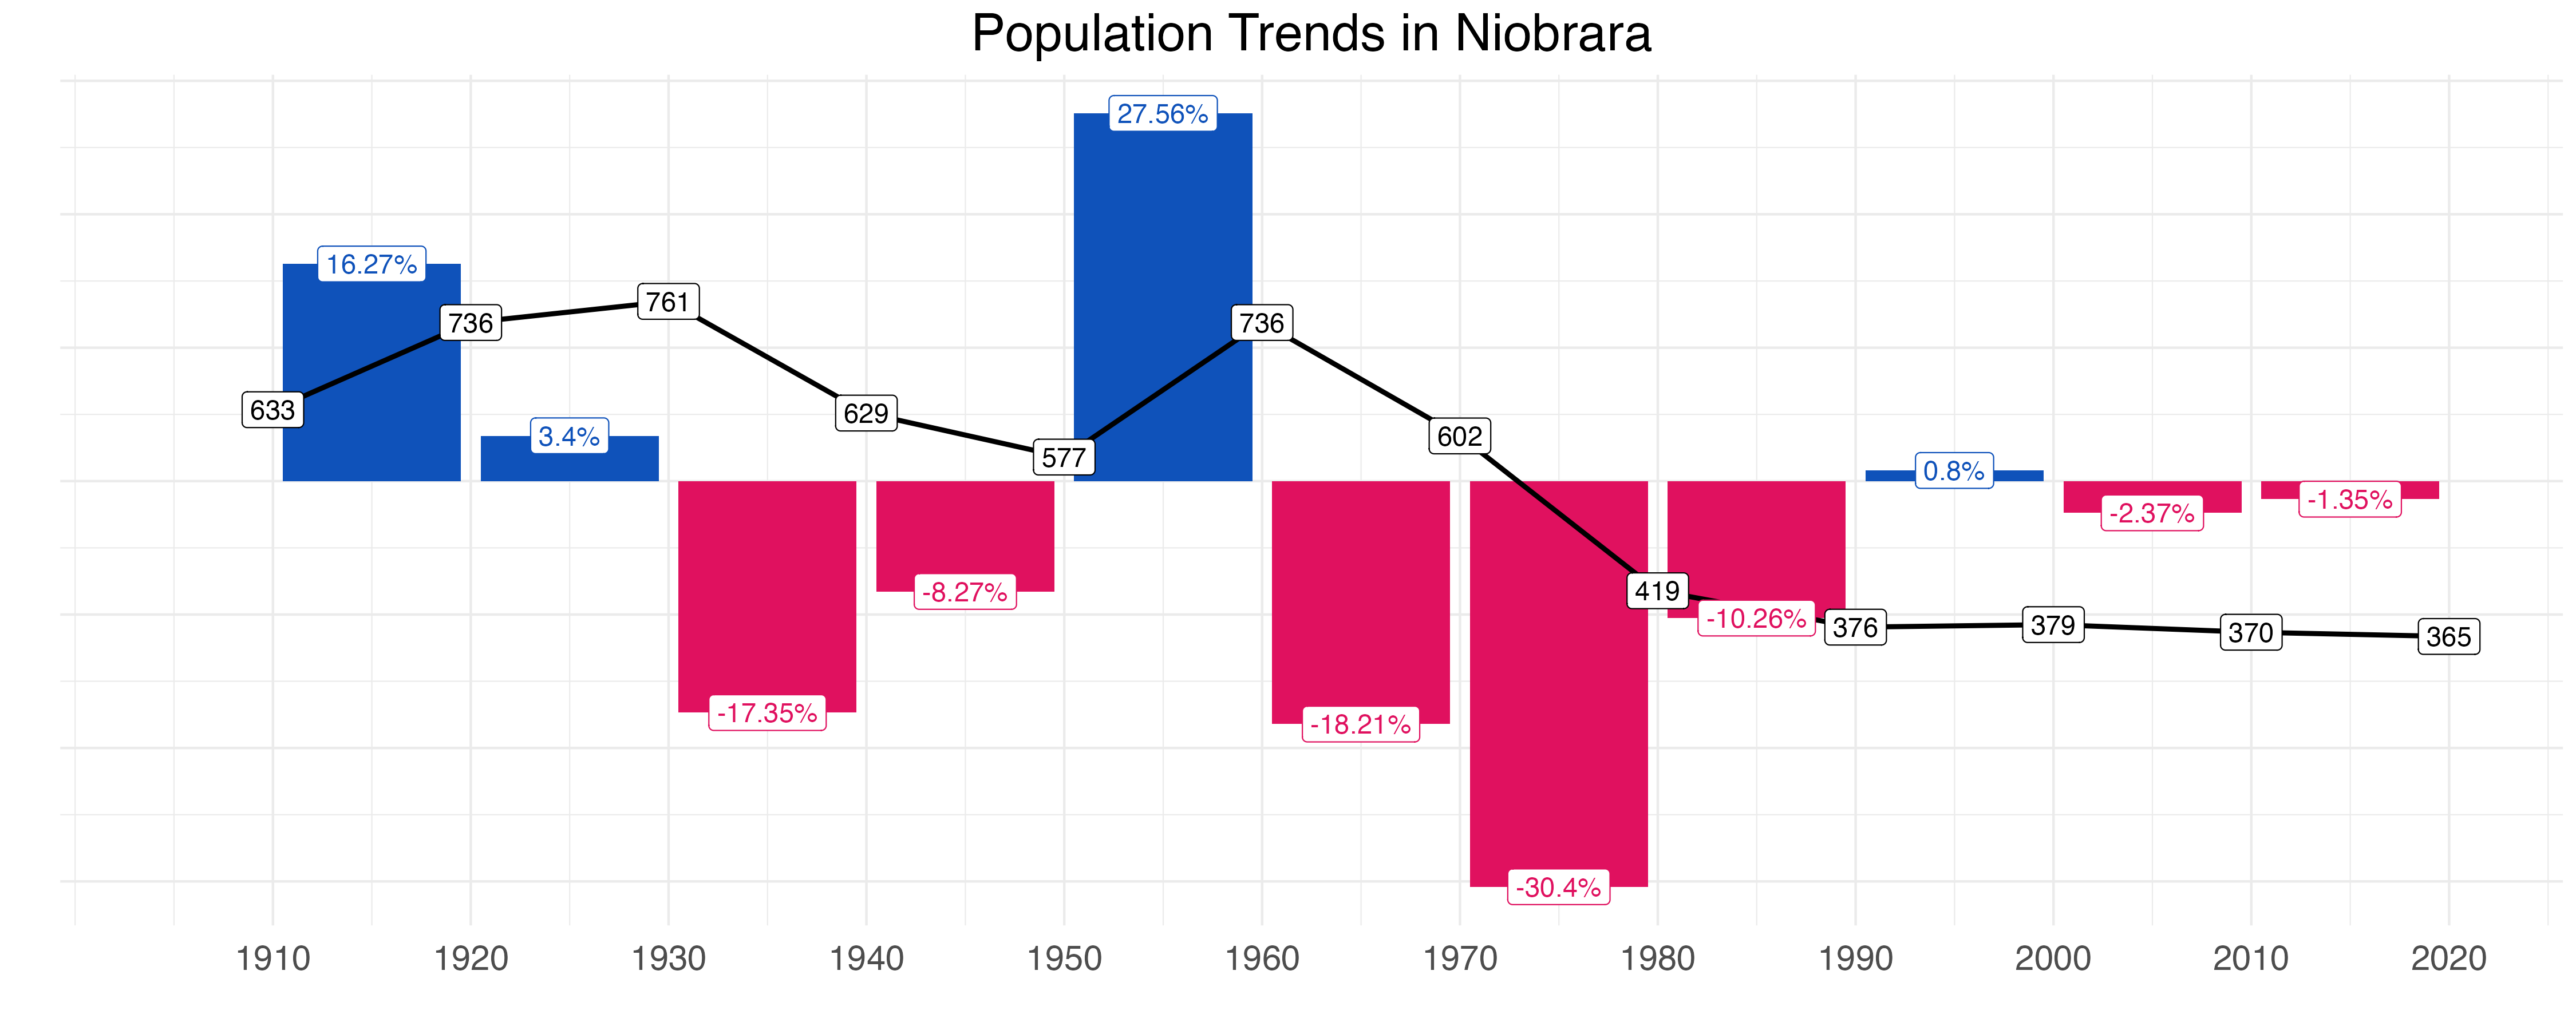
\includegraphics[keepaspectratio]{figures/historical_trends/Niobrara.png}}
\end{center}

We present several possible population scenarios for Niobrara. They
range from one-percent annual growth over the next 25 years to
one-percent annual decline. Although many factors -- some outside of the
control of Niobrara residents -- influence which scenarios will become
reality, many communities express that a target scenario of 0.25\%
annual growth is a policy goal. Achieving this goal will require
Niobrara to maintain and update its housing stock. Allowing the housing
stock to stagnate will make the population decline scenarios more
likely.

\begin{center}
\pandocbounded{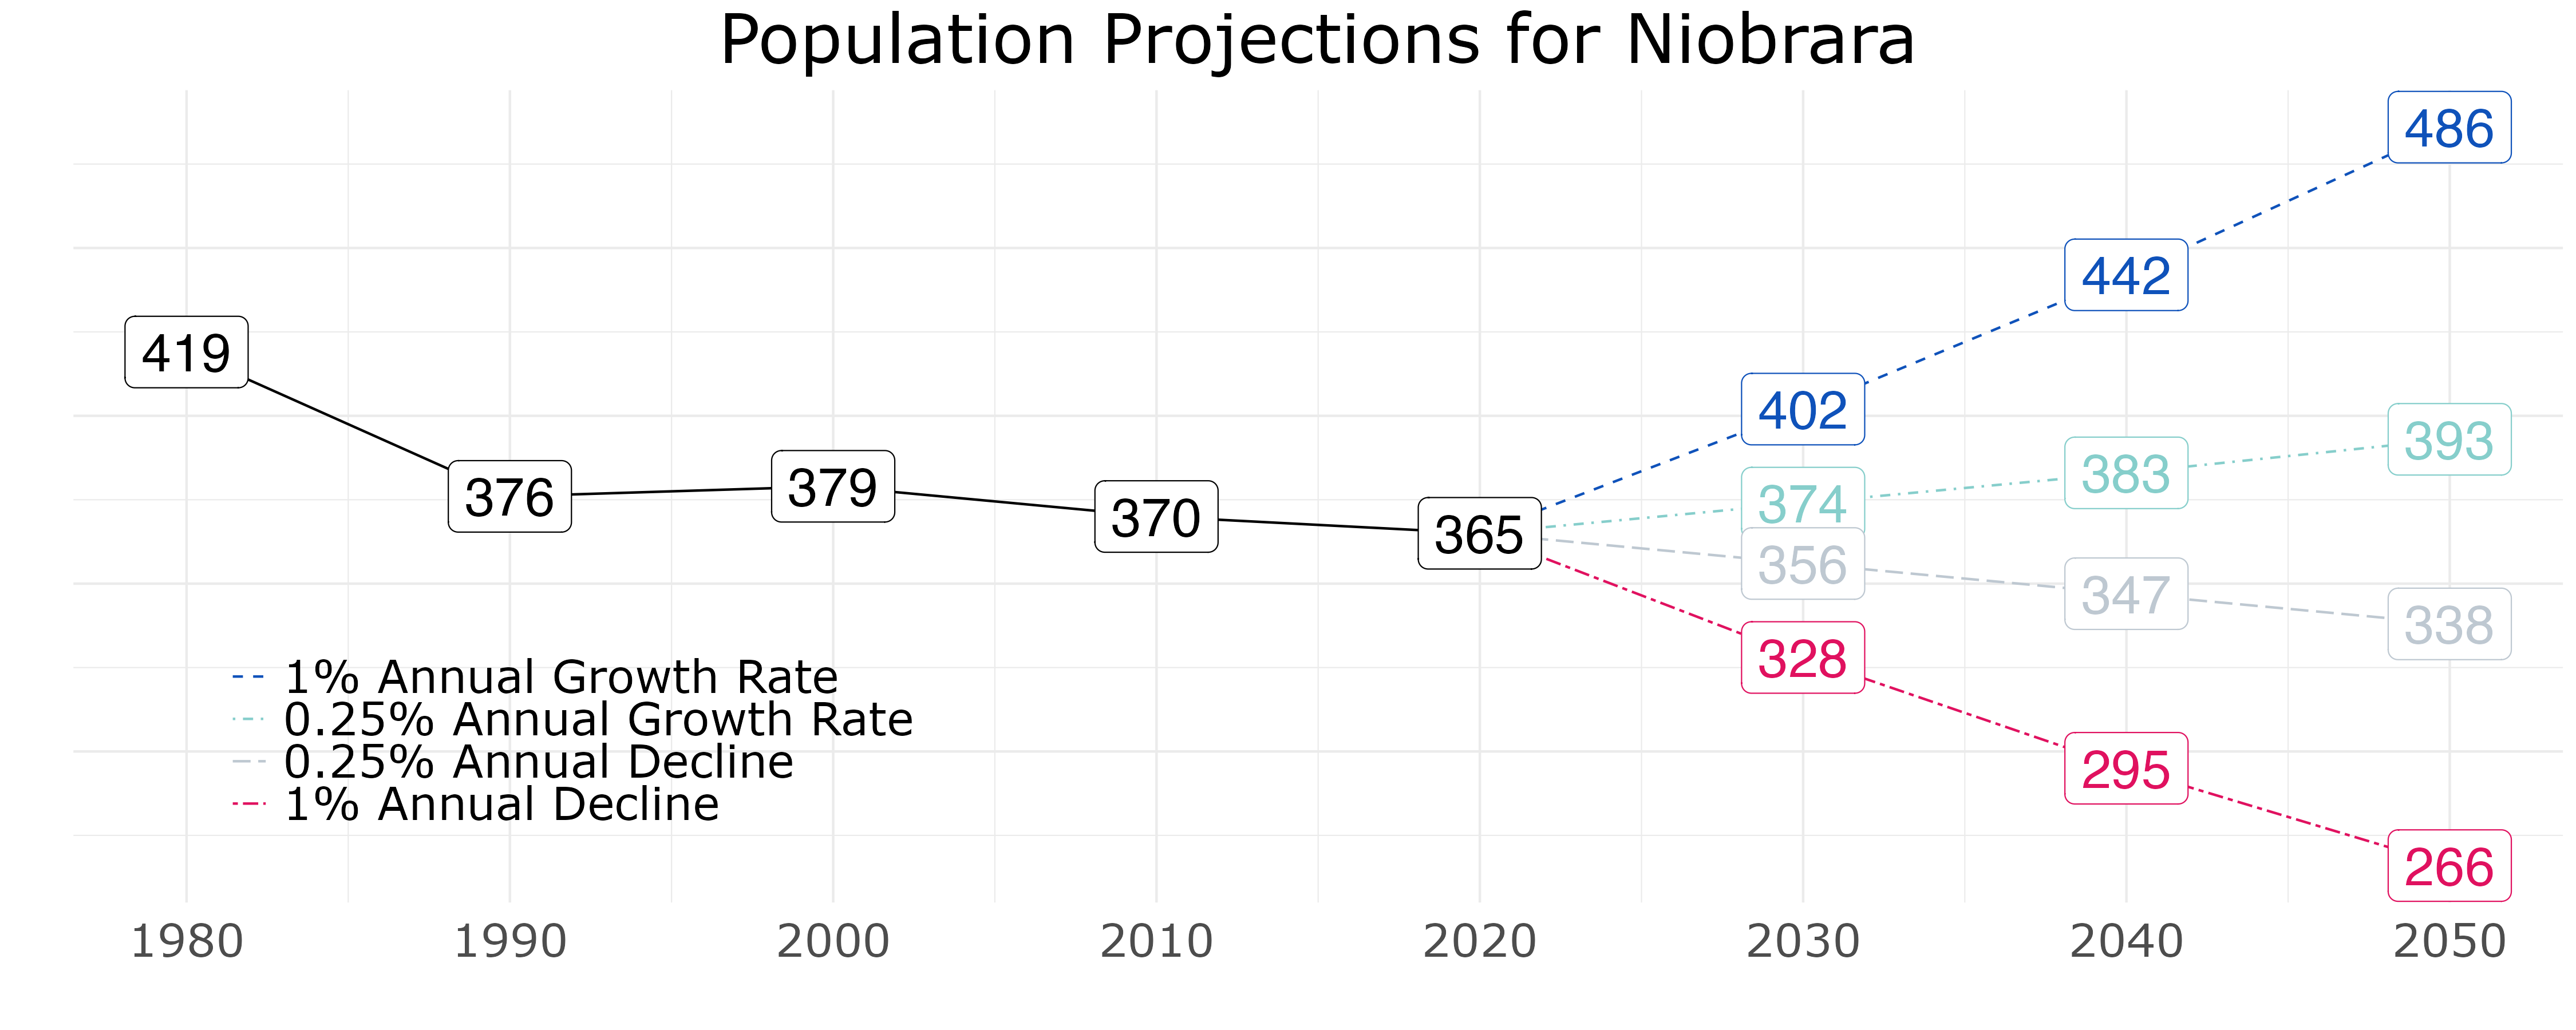
\includegraphics[keepaspectratio]{figures/pop_projections/Niobrara.png}}
\end{center}

The Census defines a family as any two or more people (not necessarily
including a householder) residing together and related by birth,
marriage, or adoption. A household consists of one or more persons
residing together who may or may not be related by birth, marriage, or
adoption. Multiple families can reside in the same household.

We show how the average family and household sizes in Niobrara have
changed -- or rather, not really changed -- over the past decade. Both
the average family size and average houehold size have increased by
marginal amounts. This makes sense given how little the Village's
overall population has changed in recent years.

\begin{center}
\pandocbounded{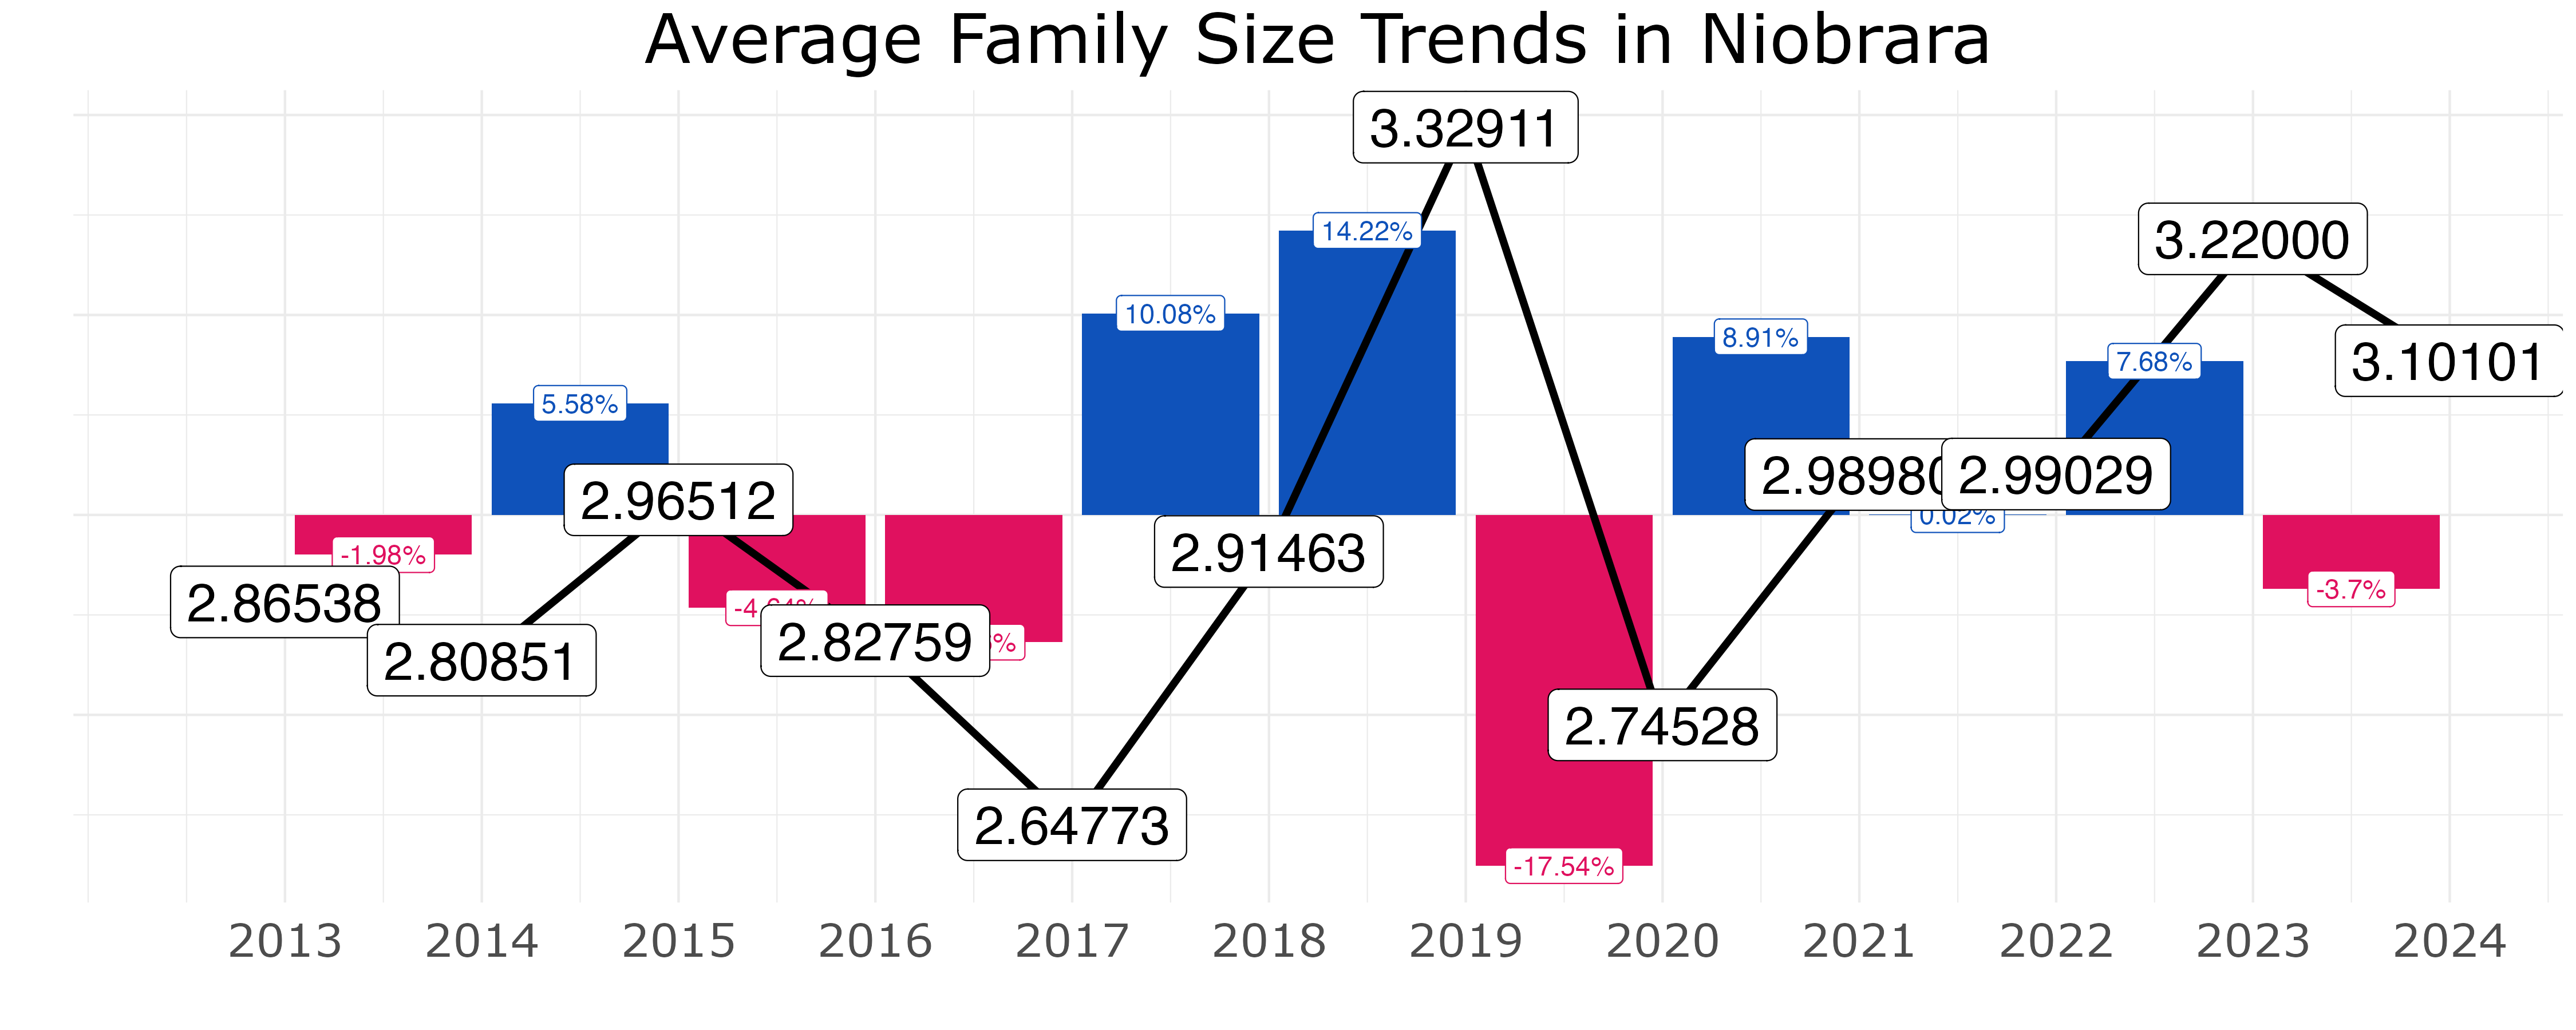
\includegraphics[keepaspectratio]{figures/hh_sizes/fam_sizes_3134370_Niobrara_NE.png}}
\end{center}

\begin{center}
\pandocbounded{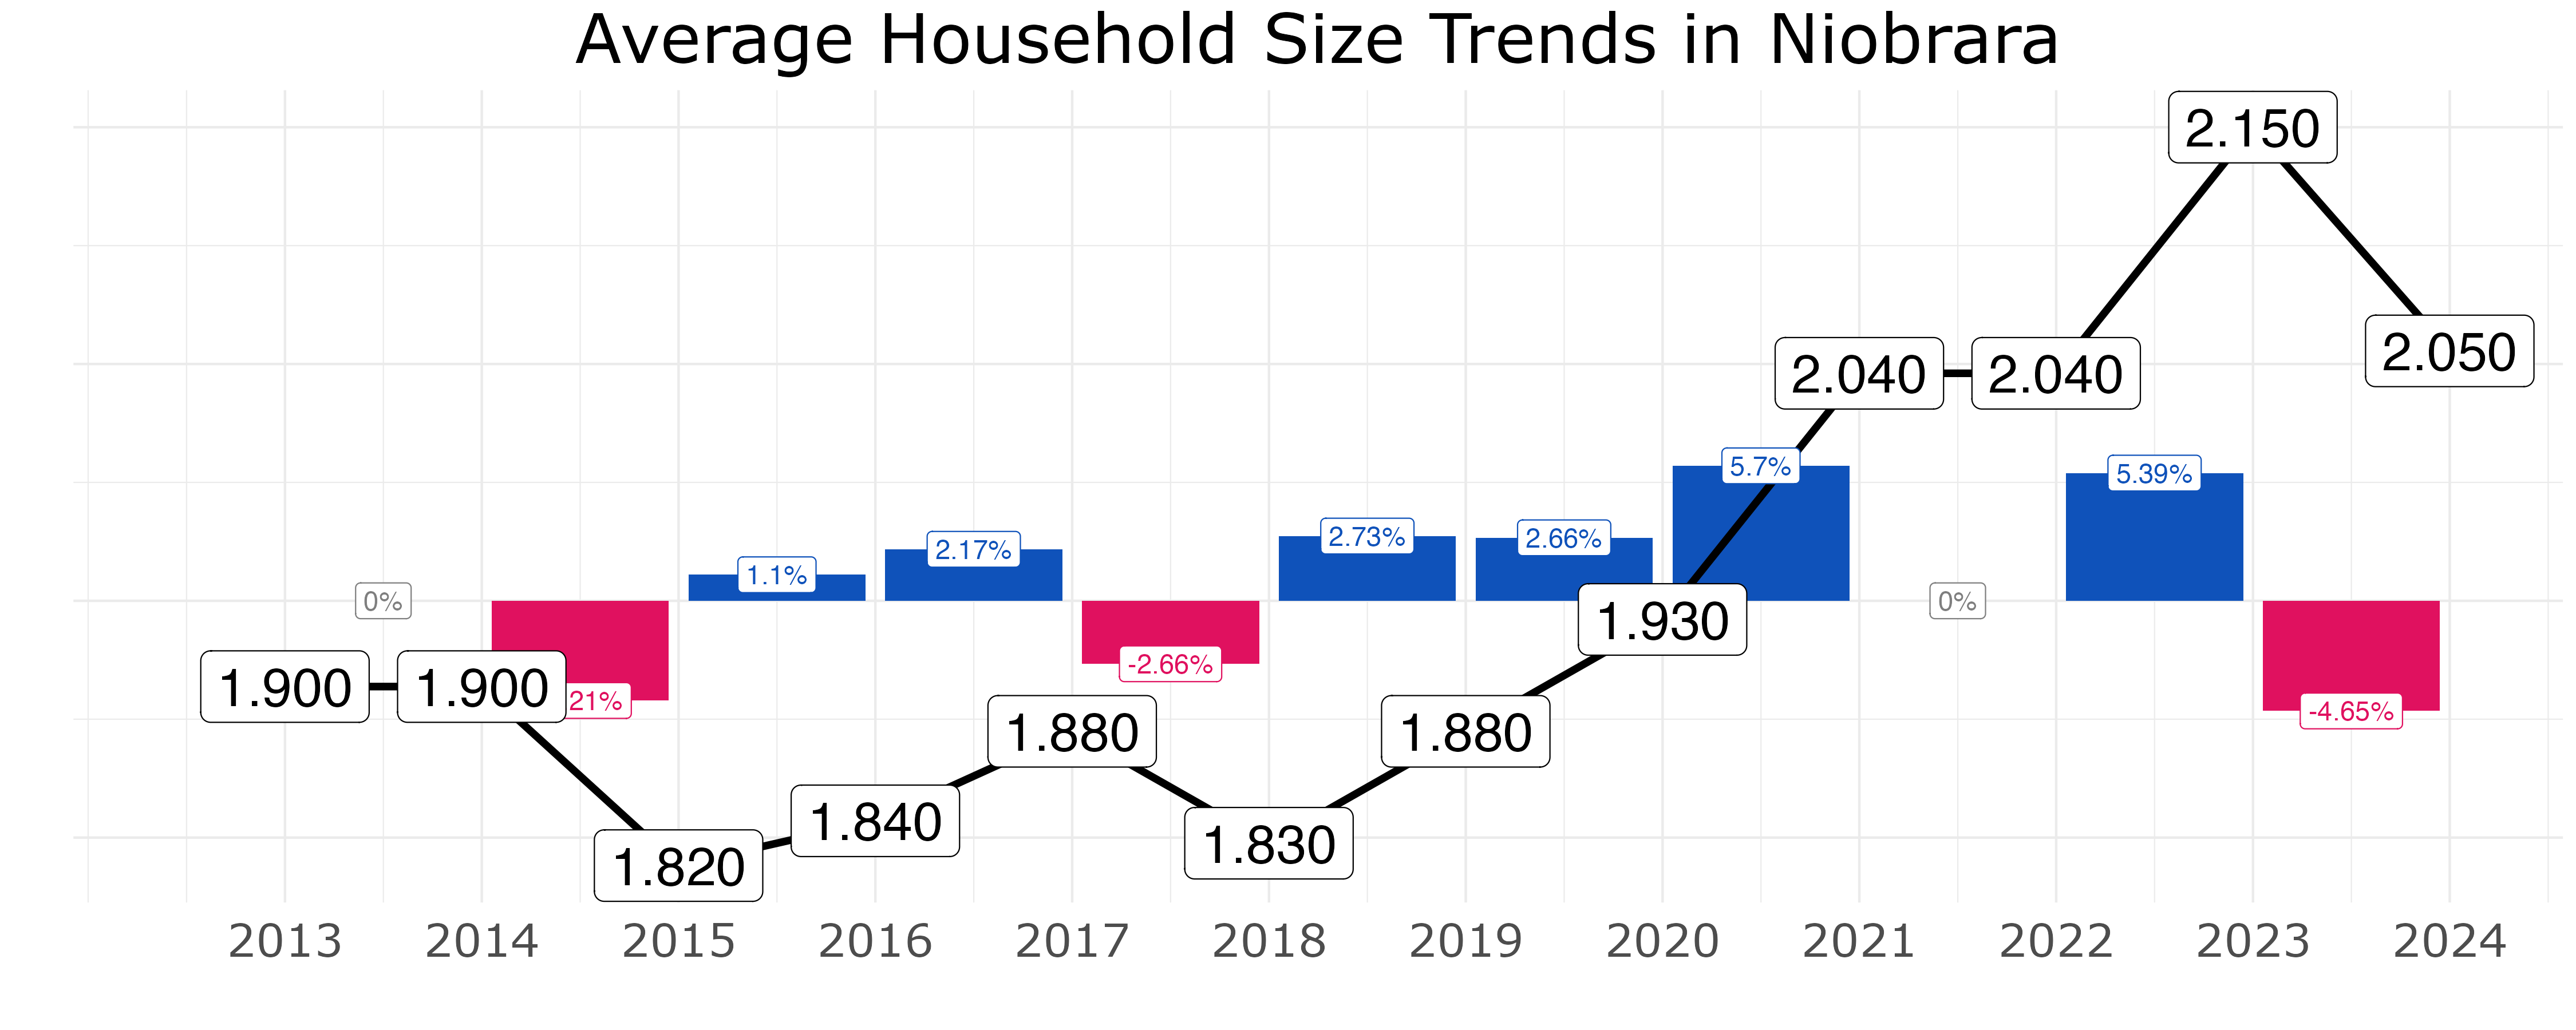
\includegraphics[keepaspectratio]{figures/hh_sizes/hh_sizes_3134370_Niobrara_NE.png}}
\end{center}

We can use these values to project Niobrara's housing needs over the
next several decades. Using the 2024 ACS estimate of 2.05 persons per
household, we estimate that, in the 0.25\% growth rate scenario Niobrara
will need 15 additional houses by 2050, or about one houses every
two-to-three years. In the more ambitious 1\% growth rate scenario,
Niobrara will need 60 additional houses, or about five houses every two
years.

These projections do not reflect the necessity of replacing aging
housing stock in Niobrara. By 2050, the majority of Niobrara homes will
be at or past half of their expected lifespan. In addition to adding new
housing units, developers and village officials need a path to turning
over existing aging units. In the extreme growth scenario, Niobrara will
likely have successfully constructed a number of new housing units where
none currently exist and have successfully renovated or replaced aging
units.

\begin{longtable*}[l]{>{\raggedright\arraybackslash}p{12em}>{\centering\arraybackslash}p{12em}>{\centering\arraybackslash}p{12em}}
\toprule
\cellcolor{gray}{\textcolor{white}{}} & \cellcolor{gray}{\textcolor{white}{1\% Annual Growth Rate}} & \cellcolor{gray}{\textcolor{white}{0.25\% Annual Growth Rate}}\\
\midrule
\endfirsthead
\multicolumn{3}{@{}l}{\textit{(continued)}}\\
\toprule
\cellcolor{gray}{\textcolor{white}{}} & \cellcolor{gray}{\textcolor{white}{1\% Annual Growth Rate}} & \cellcolor{gray}{\textcolor{white}{0.25\% Annual Growth Rate}}\\
\midrule
\endhead

\endfoot
\bottomrule
\endlastfoot
\cellcolor{gray!10}{Projected Population in 2040} & \cellcolor{gray!10}{442} & \cellcolor{gray!10}{383}\\
Projected Population in 2050 & 486 & 393\\
\cellcolor{gray!10}{Population Increase by 2050} & \cellcolor{gray!10}{121} & \cellcolor{gray!10}{28}\\
\cellcolor{gray}{\textcolor{white}{New Housing Units Needed by 2050}} & \cellcolor{gray}{\textcolor{white}{60}} & \cellcolor{gray}{\textcolor{white}{15}}\\*
\end{longtable*}

Niobrara community leaders should also pay close attention to the
community's demographic distribution when prioritizing housing
strategies.

\pandocbounded{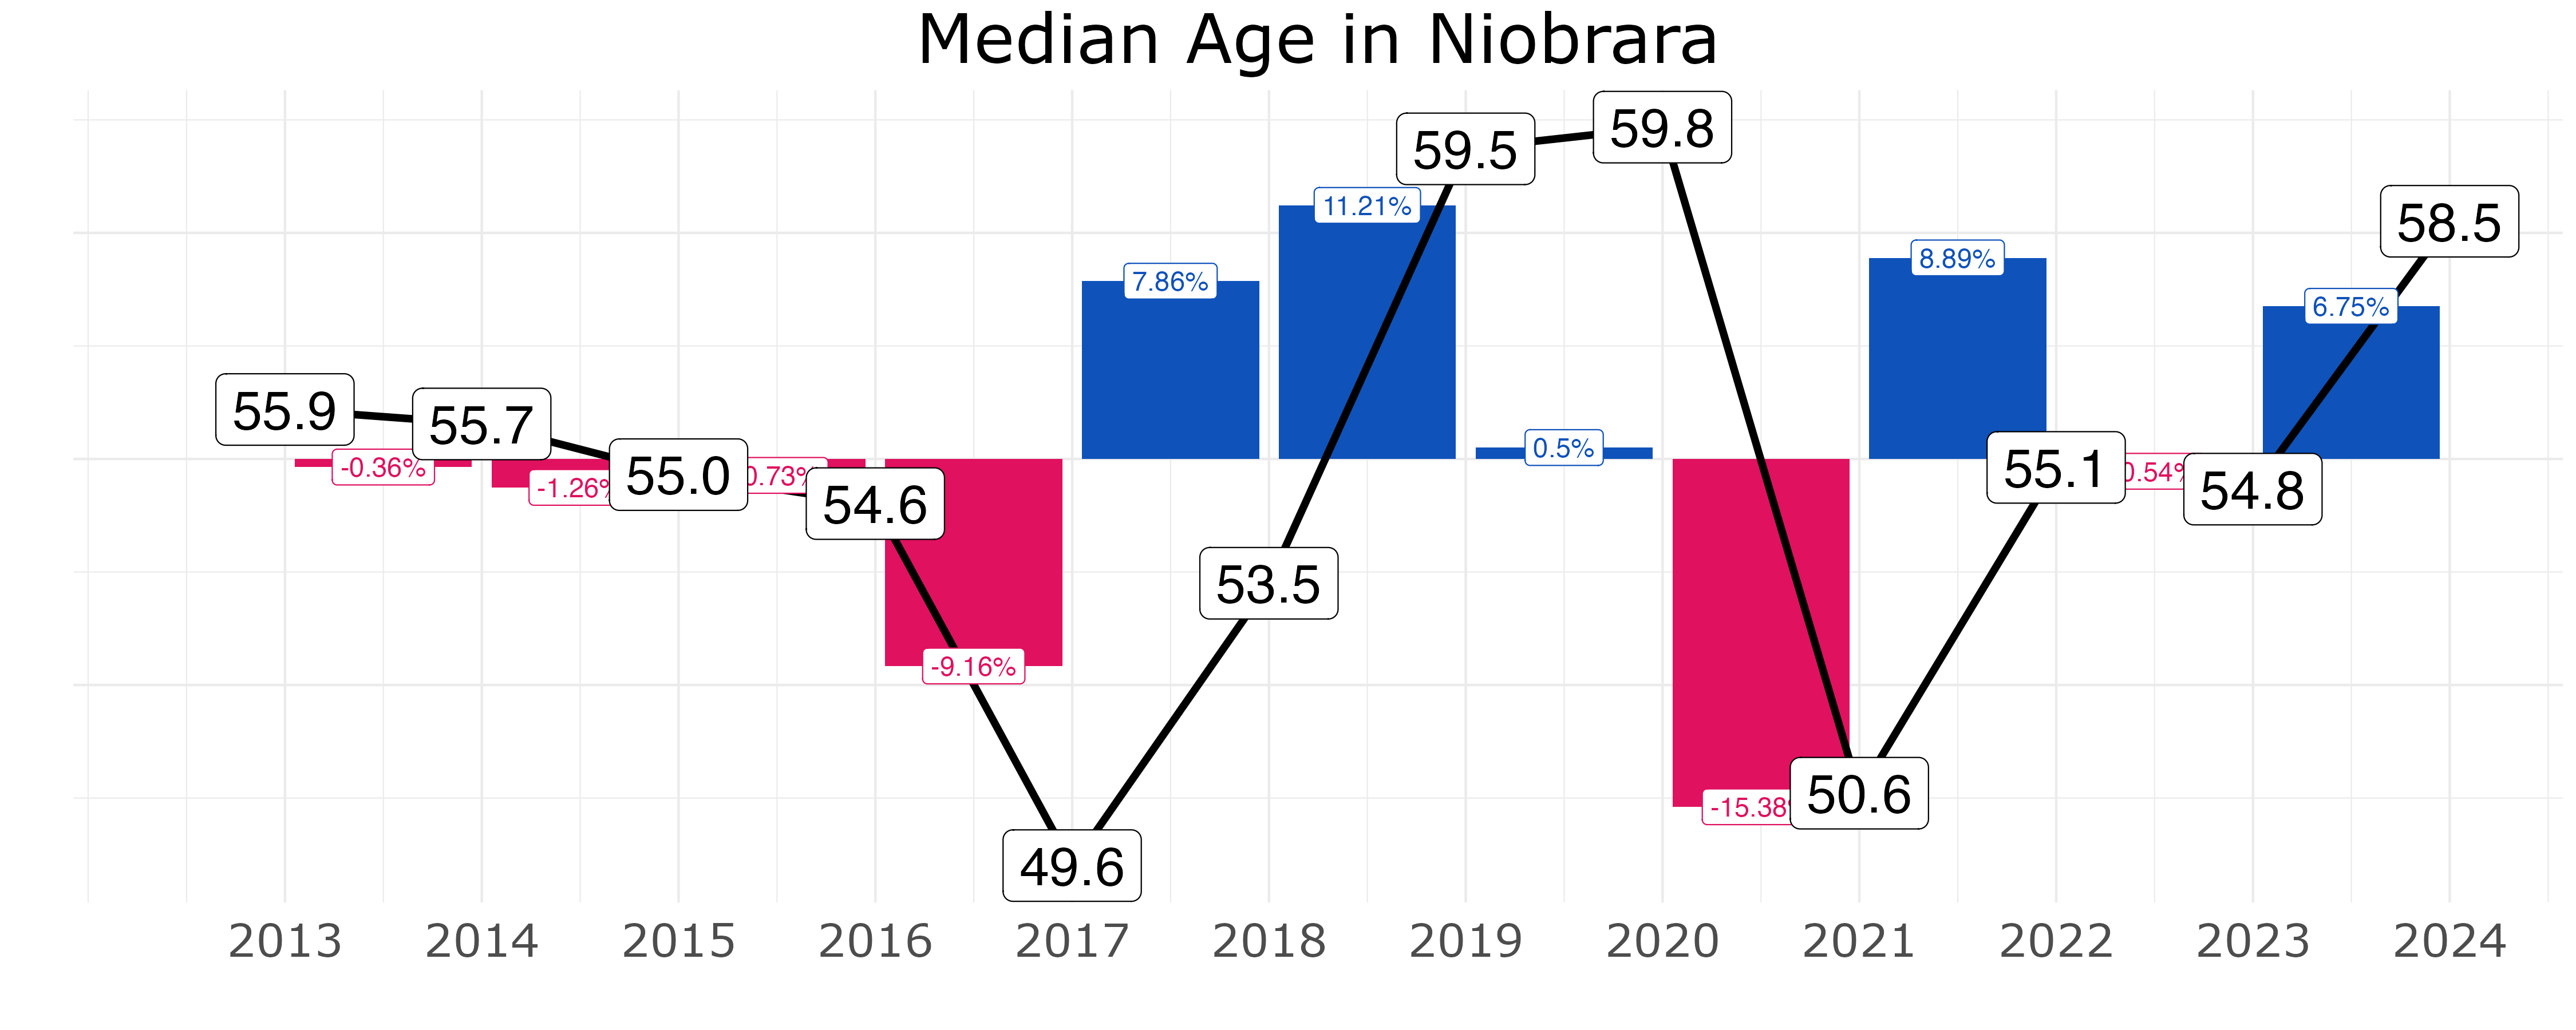
\includegraphics[keepaspectratio]{figures/median_age/median_age_3134370_Niobrara_NE.png}}

\pandocbounded{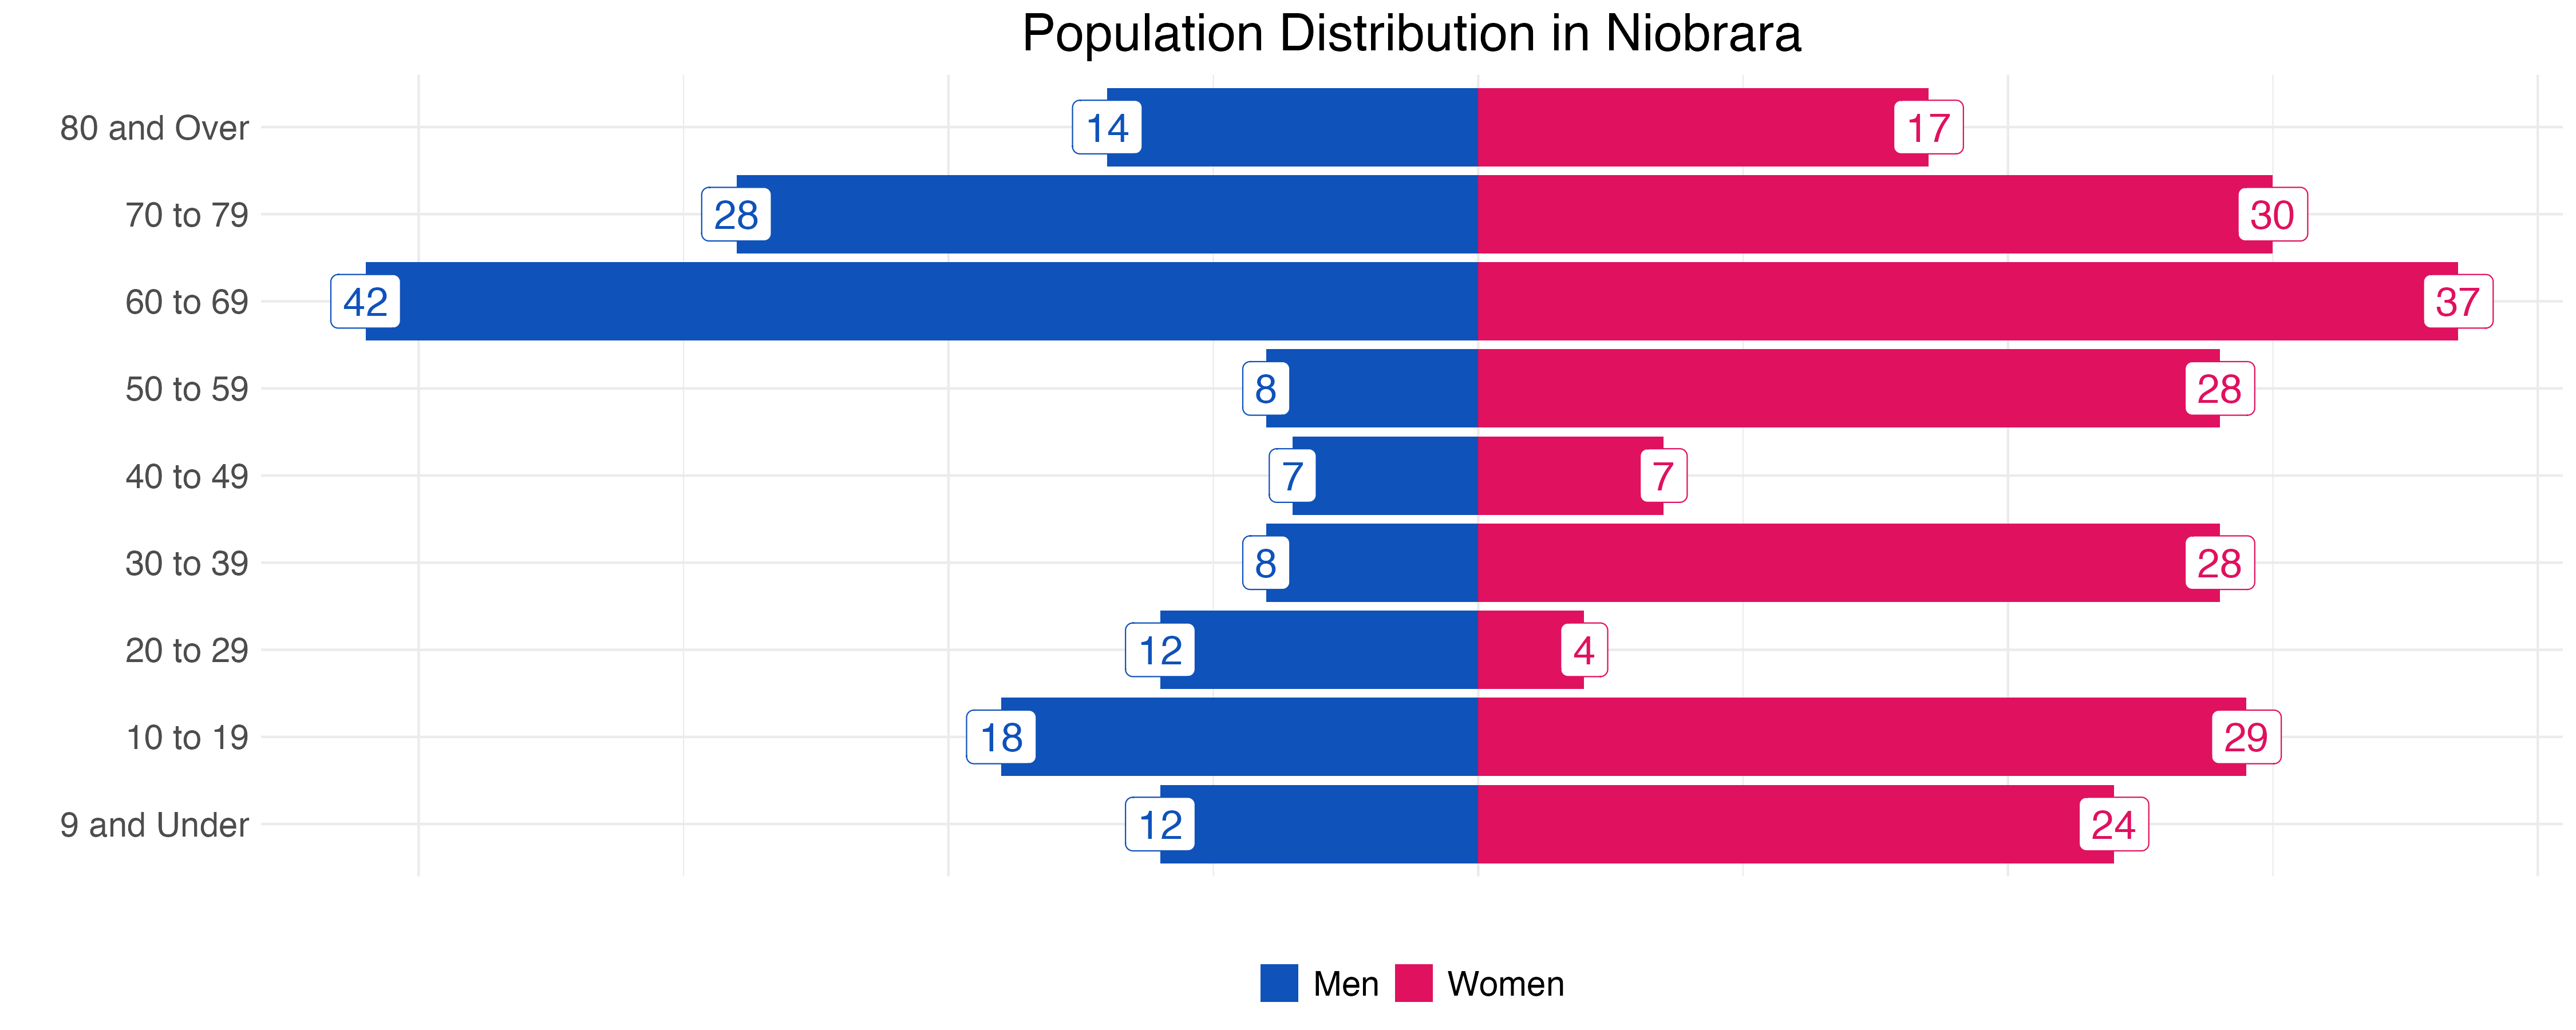
\includegraphics[keepaspectratio]{figures/pop_pyramids/3134370_Niobrara_NE.png}}

Based on American Community Survey data, the village has a healthy share
of residents over the age of 60. If (or as) the share of Niobrara's
residents continues to age, Niobrara homeowners should ensure that homes
and public facilities maintain accessibility. Furthermore, if the
village is to attract or maintain younger cohorts, it may be wise to
pursue the construction of new (and rehabilitation of existing)
single-family homes.

\subsection*{Affordable Housing
Assessment}\label{affordable-housing-assessment}
\addcontentsline{toc}{subsection}{Affordable Housing Assessment}

The affordability and accessibility of housing at the right value are
paramount. Census data indicate that home values in Niobrara have slowly
risen over the past decade. Unfortunately, household incomes have
actually fallen over that same time span, possibly due to flooding in
2019 or the COVID-19 pandemic. This indicates that more Niobrara
residents, on average, risk being priced out of being able to purchase
new homes.

\pandocbounded{
\includegraphics[keepaspectratio]{figures/hh_costs/hh_costs_3134370_Niobrara_NE.png}}

Finally, we show that the current housing inventory is not suited to the
income distribution of Niobrara residents. In general, a home is
affordable if its value is no more than twice the household income of
its resident. For instance, if a household's income is \$50,000, then
the value of their home should be approximately (but not more than)
\$100,000. We find that Niobrara has a shortage of 31 units for
households eraning at the median income.

\pandocbounded{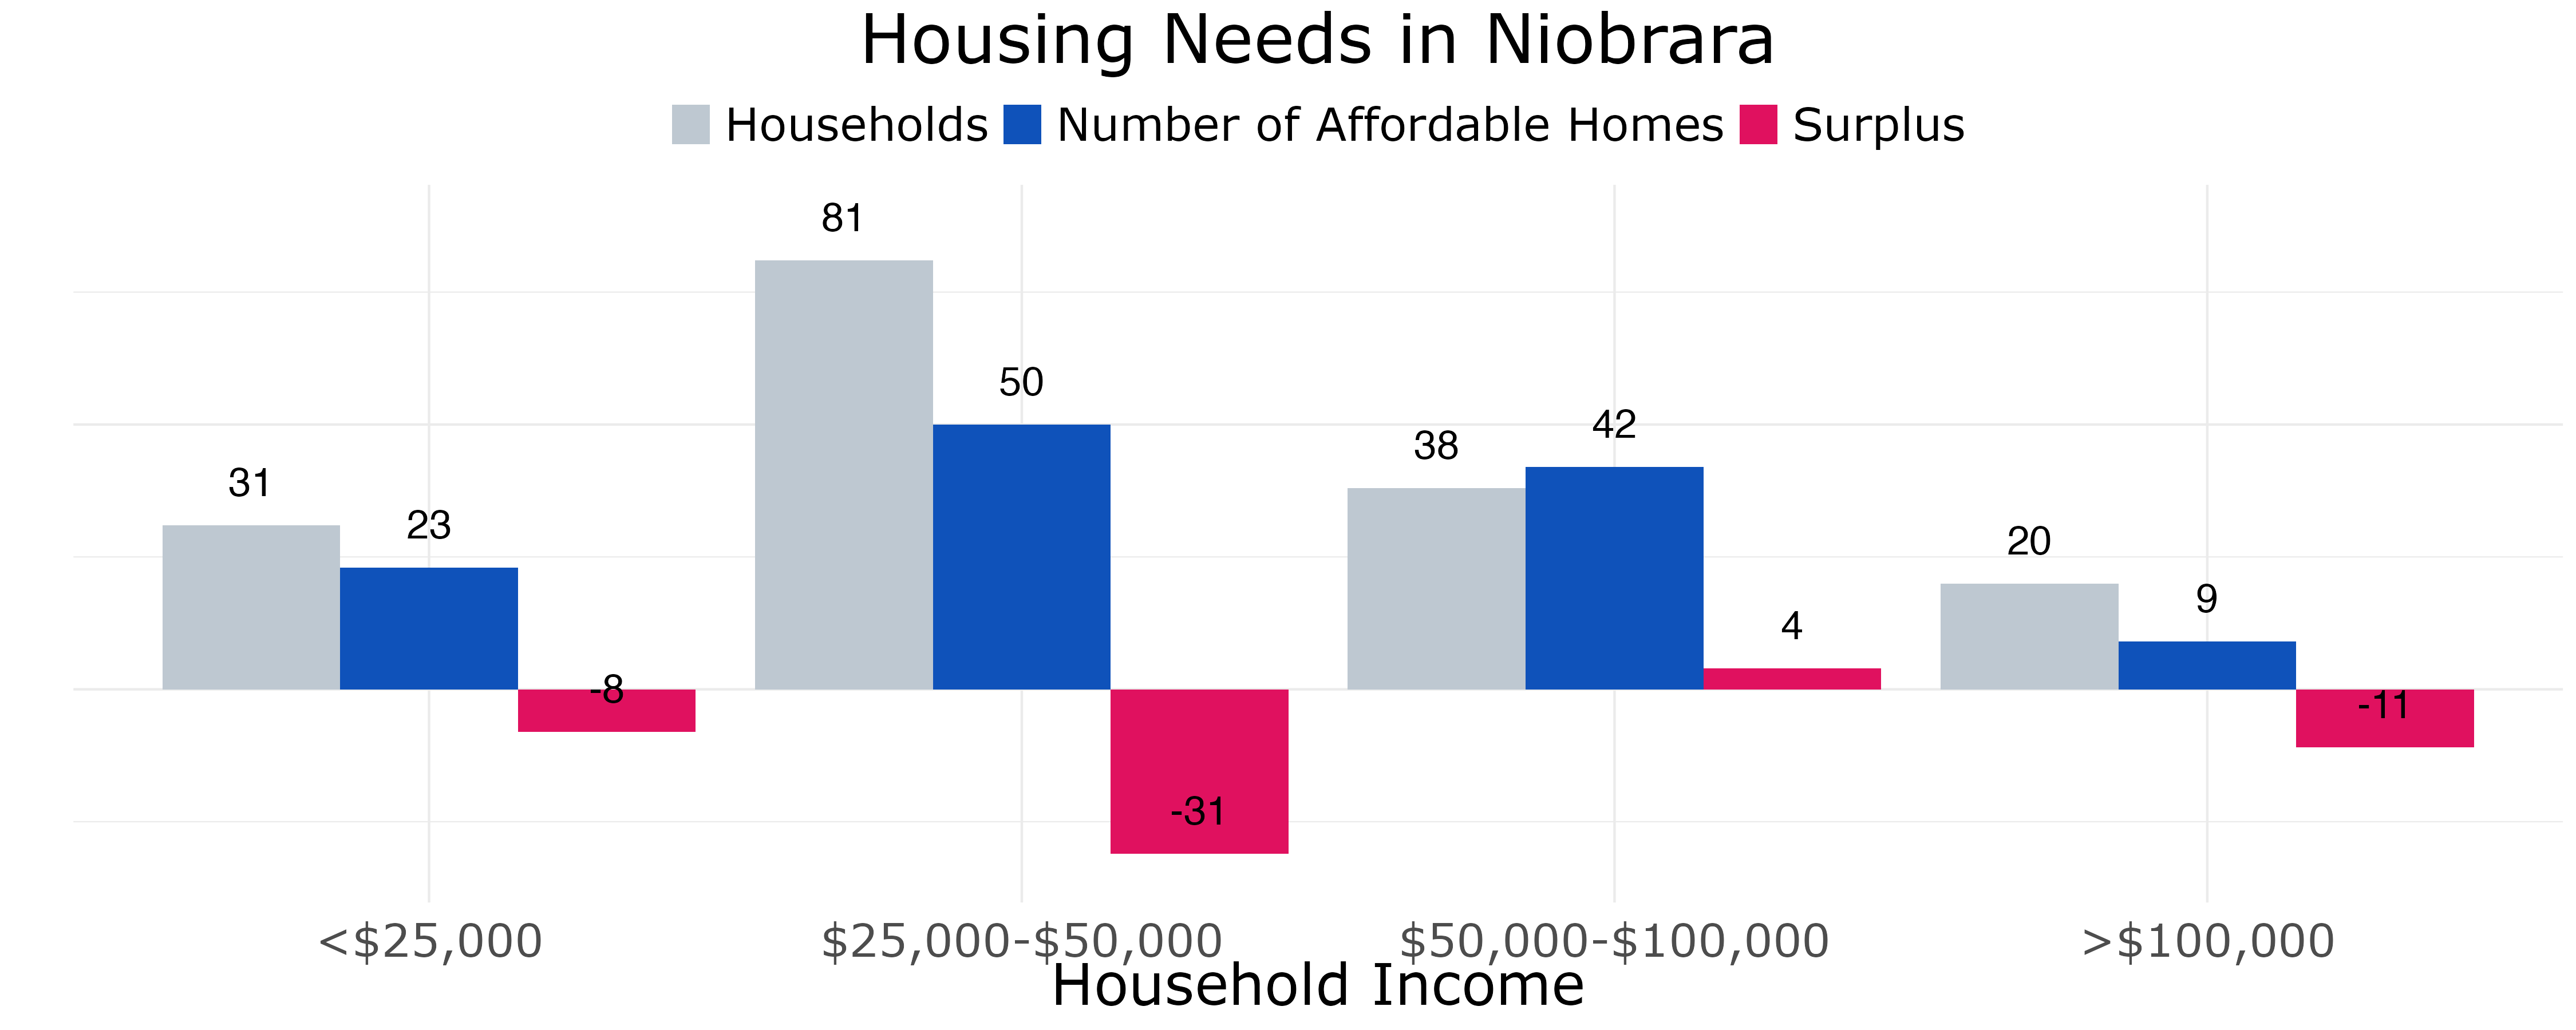
\includegraphics[keepaspectratio]{figures/hh_needs/hh_needs_3134370_Niobrara_NE.png}}

Therefore, when pursuing new housing development, Niobrara needs to
emphasize homes whose values address the shortage at the median of the
income distribution. While they homes can be costly to produce, doing so
will go a long way to remedying the general imbalance between home
values and household income capacities.

\subsection*{Appendix}\label{appendix}
\addcontentsline{toc}{subsection}{Appendix}

There are three kinds of data used to generate this Housing Study:
community engagement data, socioeconomic data, and map and geospatial
data. This appendix documents how these data were acquired, processed,
and presented. Finally, it also summarizes the technical procedures used
to generate the tangible document of the study.

Please refer any technical questions to
\url{jordan@fiveruleplanning.com}.

\subsection*{Community Engagement
Process}\label{community-engagement-process}
\addcontentsline{toc}{subsection}{Community Engagement Process}

{[}we haven't done this yet{]}

\subsection*{Socioeconomic Data
Curation}\label{socioeconomic-data-curation}
\addcontentsline{toc}{subsection}{Socioeconomic Data Curation}

FIVE RULE Rural Planning curated data from a number of sources. In
addition to the Community Engagement portion (above), we collected data
from the following sources:

\begin{enumerate}
\def\labelenumi{\arabic{enumi}.}
\tightlist
\item
  2025 U.S. TIGER/Line Shapefiles.
\item
  The Knox County, Nebraska Property Assessor.
\item
  The University of Nebraska-Omaha Data Center.
\item
  The Decennial Census.
\item
  The 2013 through 2023 American Community Survey Five-Year Estimates.
\end{enumerate}

\subsection*{Map Generation}\label{map-generation}
\addcontentsline{toc}{subsection}{Map Generation}

We relied primarily on two softwares to generate maps for this document.
For the shapefile generation and curation, we used
\href{https://www.r-project.org}{R Version 4.5.1} and the
\href{https://positron.posit.co/about.html}{Positron IDE 2026.06.0 Build
211}.

\subsection*{Document Generation}\label{document-generation}
\addcontentsline{toc}{subsection}{Document Generation}

This document was compiled and generated using the
\href{https://quarto.org}{Quarto} publishing sytem. All of the source
code can be found at the accompanying
\href{https://github.com/five-rule-planning/2026-Niobrara-Housing-Study}{GitHub
page}.

\subsection*{About the Authors}\label{about-the-authors}
\addcontentsline{toc}{subsection}{About the Authors}

\subsubsection*{Bobbi Pettit, AICP}\label{bobbi-pettit-aicp}
\addcontentsline{toc}{subsubsection}{Bobbi Pettit, AICP}

Bobbi has more than 25 years of experience working with plan creation,
plan implementation, and economic development projects across rural
Nebraska and Kansas.

Bobbi grew up in Merna, Nebraska, and has experienced firsthand what
it's like to live in a small town. Her passion for helping rural
communities runs deep. She founded FIVE RULE Rural Planning (FRRP), in
2018. She earned a Master of Arts in Community \& Regional Planning from
the University of Nebraska-Lincoln and has been a member of the American
Institute of Certified Planners (AICP) since 2011.

Before starting FRRP, Bobbi served as Assistant Development Services
Director, City of Kearney; Community Planner, South-Central Economic
Development District (SCEDD); Deputy Master Planner, Nebraska Military
Department; and 3rd District Staffer for Congressman Tom Osborne.

During her tenure with the City of Kearney, Bobbi oversaw the Planning
Commission, Development Review Team, and Chief Building Official. In
2009, Bobbi led 50 troops to Camp Liberty, Iraq, as a Platoon Leader for
the Nebraska Army National Guard.

\subsubsection*{Jordan Duffin Wong, Ph.D}\label{jordan-duffin-wong-ph.d}
\addcontentsline{toc}{subsubsection}{Jordan Duffin Wong, Ph.D}

Jordan brings eight years of cutting-edge computational social science
and spatial econometric training to the FIVE RULE team, applying his
expertise to curating planning documents for Nebraska communities.

Jordan grew up in Kearney, Nebraska, and returned to join FRRP in the
summer of 2025. Before, Jordan held positions with Washington University
in St.~Louis, the Weidenbaum Center on the Economy, Government, and
Public Policy, the St.~Louis Zoning Atlas, and the Nebraska Bureau of
Business Research (BBR).

At BBR, Jordan was a contributor on the inaugural Rural Prosperity
Nebraska Thriving Index, and has co-authored numerous scholarly articles
on local government, published in both peer-reviewed journals and
academic conference proceedings.

Jordan completed two Bachelor of Arts Degrees, in Economics and in
Political Science, from the University of Nebraska-Lincoln in 2020, with
a minor in Mathematics. In 2025, Jordan completed his Master of Arts and
Doctor of Philosophy (Ph.D.), both in Political Science, at Washington
University in St.~Louis. His classroom experience includes teaching and
tutoring a variety of Mathematics, Political Science, and Statistics
courses.




\end{document}
